\section{Background}\label[sec]{background}
Micro Areal Vehicles (MAVs) have great potential in contributing to indoor search and rescue missions. Their small size and weight
make them easy to transport and allows for rapid field deployment. Furthermore they are agile, allowing them to operate in 
complex environments and accessing hard-to-get-to places.

Limitations of current technologies, prohibiting the existance of fully autonomous MAVs, are examined in \cite{MAV_enabling}. They define the following
requirements for a fully autonomous MAV:
\begin{itemize}
  \item Inference: The ability to infer situational awareness from sensory measurements.
  \item Reasoning: The ability to define a mission based on abstract human-defined goals.
  \item Unsupervised learning: The ability to adapt and learn its own controll strategies without human supervision.
\end{itemize}
Due to the constraints on the size of MAVs, the existance of fully autonomous MAVs are mainly dependent on the existance of 
small and efficient enough hardware components such as power supplies, sensors and processors allowing them to quickly process the incoming data and convert them to actions.
In \cite{MAV_enabling} they conclude that as of March 2017 no fully autonomous MAV system exist.

Although a fully autonomous MAV system is yet to be realised, the advancement in transistor density shown in \figref{trans_density}, and continously dimishing price of microprocessors continue to
allow for faster, and thus more complex, on-board computations. This allows for increased level of autonomy of the MAVs as they can perform ever
more complex computations locally without the aid of other computation units or human interference.
\begin{figure}[H]
  \centering
  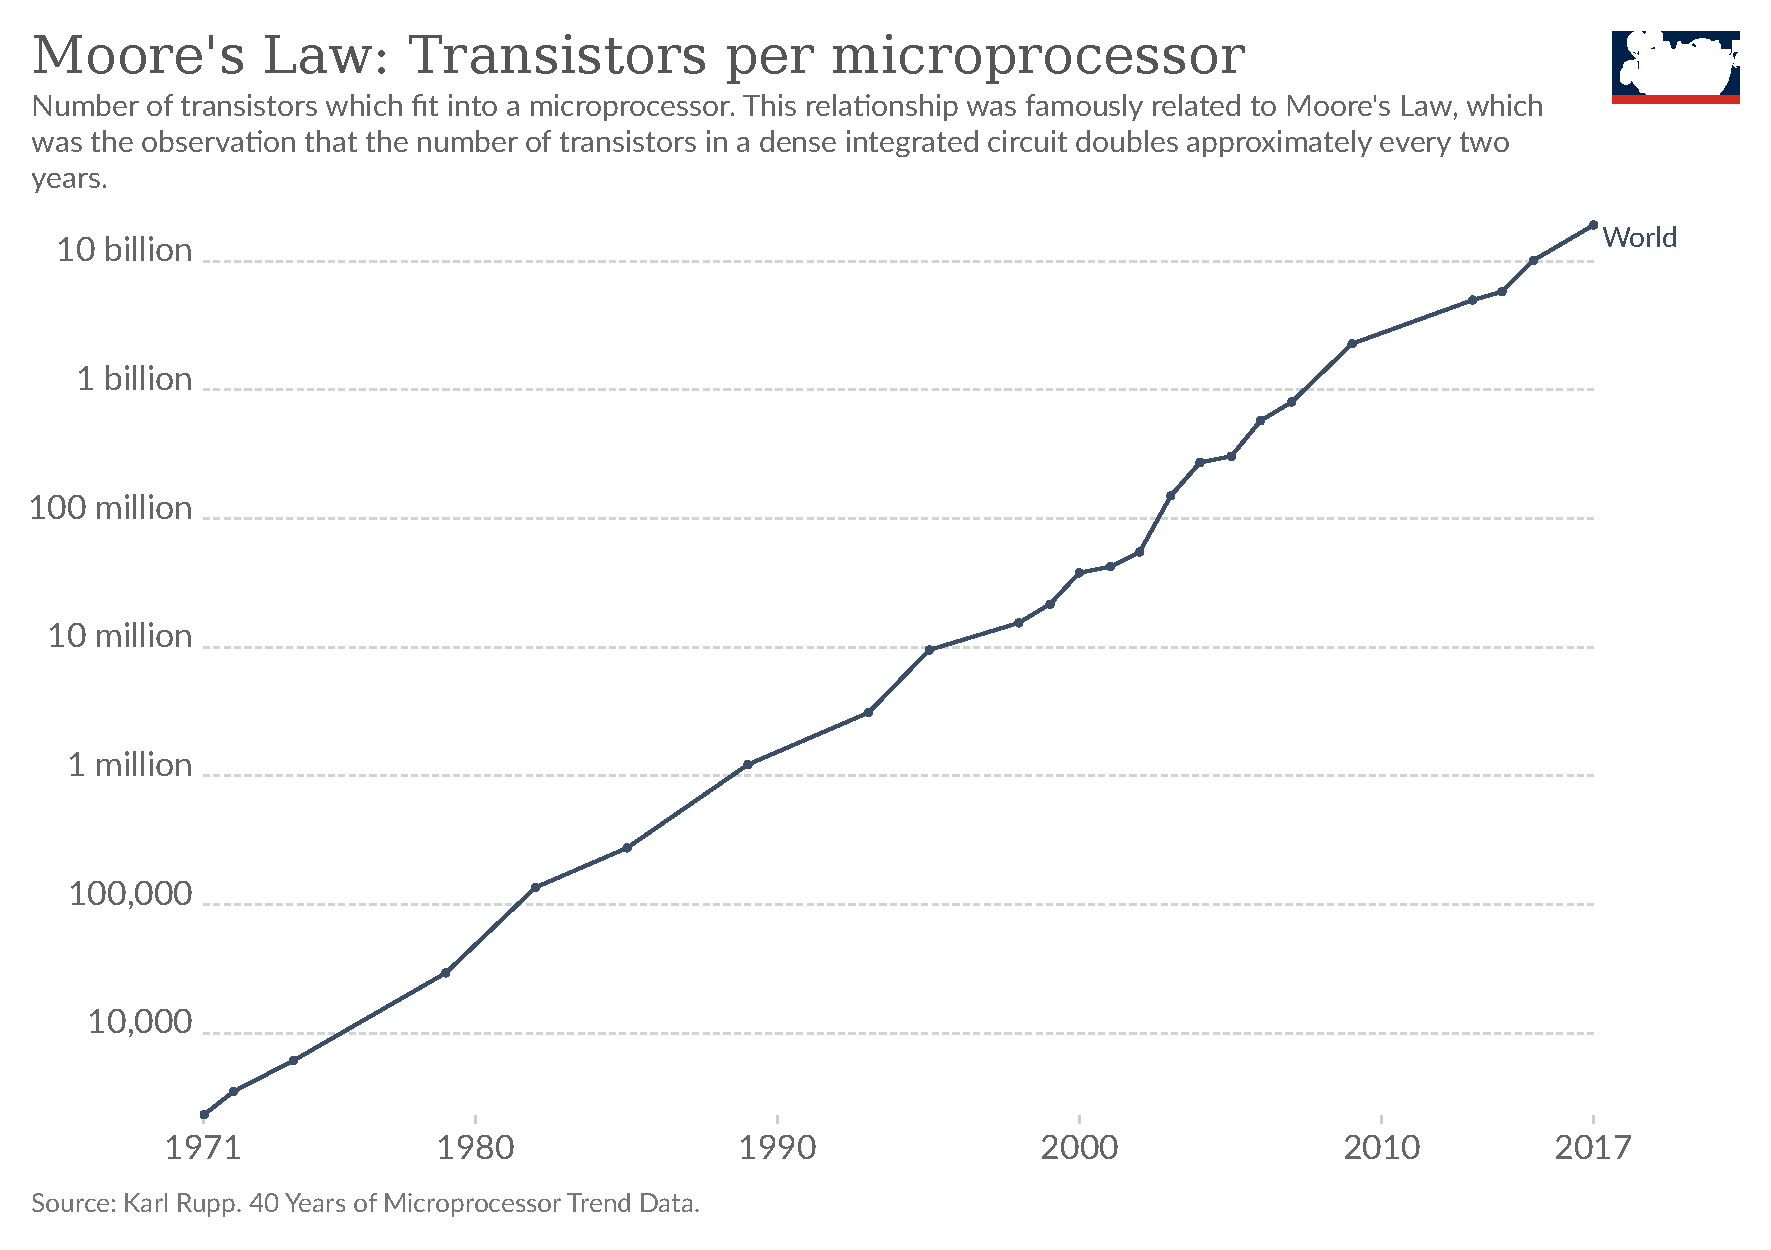
\includegraphics[width=.6\textwidth]{figs/transistors-per-microprocessor.pdf}
  \caption{Evolution of number of transistors per microprocessor.}
  \label[fig]{trans_density}
\end{figure}
Most MAVs utilize electrical propulsion systems as they are easier to miniaturize, and have faster response time than combustion based systems. Energy is typically stored on
LiPo batteries. \figref{lion_price} shows how the energy density and price of Lithium-ion batteries have evolved over the last decades. As the energy density of Lithium-ion batteries already have and is projected to continue to increase, this will allow 
for fitting more power consuming equipment on the MAVs, and increasing their endurance. Thus enabling MAVs to take on more complex and long lasting missions, resulting in an increasing autonomy.
\begin{figure}
  \centering
  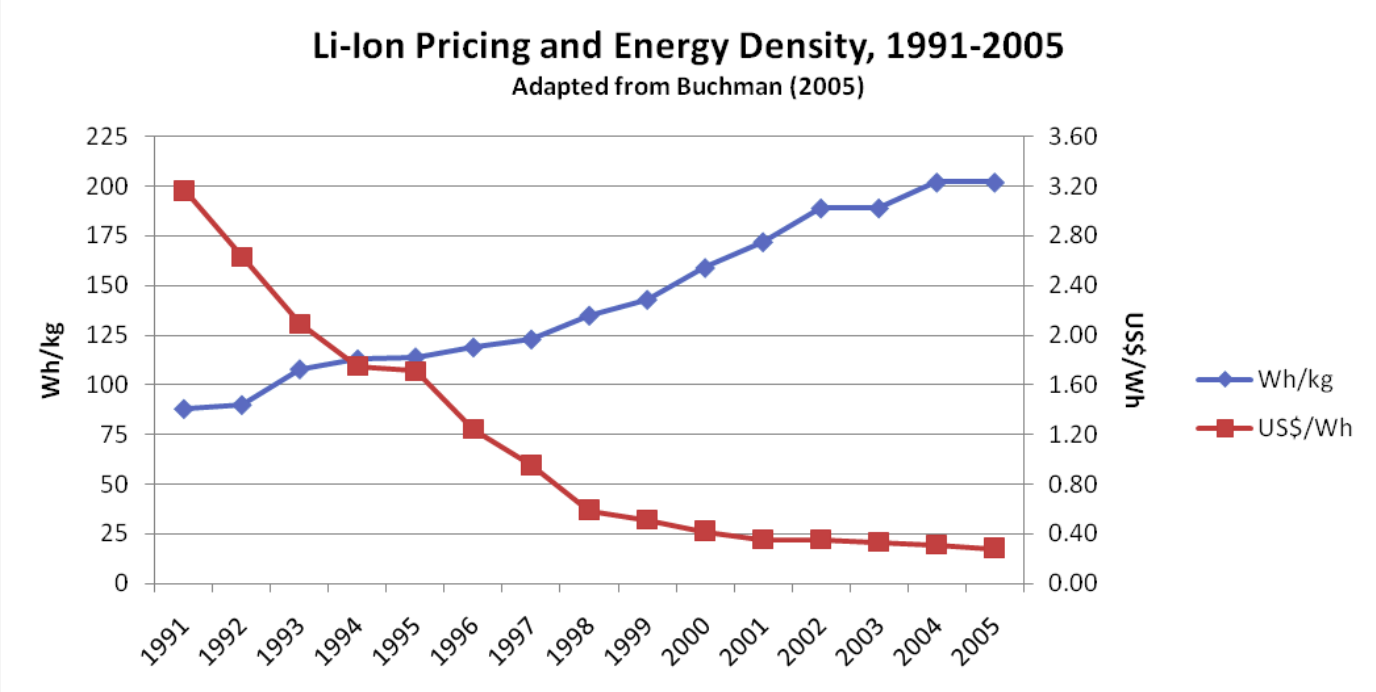
\includegraphics[width=.6\textwidth]{figs/lion-price.png}
  \caption{Evolution of energy density and cost of Lithium-ion batteries. Source: \cite{lion}.}
  \label[fig]{lion_price}
\end{figure}

Not only hardware components have made leaps over the last decades. The advancement in autonomy of MAV systems has been a field of great scientific interest.
The Robotics \& Perception Group at the University of Zurich have performed excessive research into the field of visual-inertial based real-time navigation and mapping
by MAVs in GNSS denied environments \cite{svo2, svo1}. The goal of which is enabling MAVs to localize themselves in and map unknown environments without external aid.

In \cite{svo2} a fast and robust visual-odometry algorithm (SVO) is presented. The method is faster than previously presented methods, and is therefore especially usefull 
for MAV operations as it should be able to run on a onboard computer with limited processing power. It is concluded that the method is especially usefull for state estimation onboard MAVs as the algorithm runs
at a high enough rate to provide accurate state estimates. Furthermore the use of depth-filters yields an accurate map of the environment with few outliers.

In \cite{svo1} Scaramuzza et al. present a system for autonomous mapping of unknown indoor and outdoor environments performed by a single MAV using SVO. The MAV is supplied with 
a trajectory it is to follow, and using only on-board processing and sensing follows said trajectory and provides at the same time a real-time map of the environment.

A lot of research has also been put into distributed swarm controll: the task of making a set of MAVs work together to fulfill some collective goal, and doing so 
with only local information. In \cite{connectivity_subgradient} De Gennaro and Jadbabaie present a distributed method for optimizing the connectivity of a multi-agent network.
In their approach each agent knows only the state of its neighbours, where another agent is defined as a neighbour if it fulfills some proximity condition.
Their approach shows through simulations that the the swarm reaches a configuration that corresponds to a maxima of the second smallest eigenvalue of the Laplacian matrix.

Cassandras and Zhong present in \cite{cassandras} a distributed method for a multi-agent network in which the goal is maximizing the joint detection probability of randomly occuring events in an unknown environment.
They also present an algorithm that preserves connecticity of the network of agents. They conclude that using their method, the swarm of agents reach a configuration corresponding to a 
local maxima of the joint detection probability function. Furthermore they find that when connecticity preservation is imposed, the swarm settles at a configuration in which the joint detection probability is
smaller than when connectivity of the network is not taken into account.

Note to self:
\begin{itemize}
  \item CrazyFlie (and other small scale drones)
  \item Increase in computational power
  \item State of the art drones
\end{itemize}